\subsection{Ejercicio 2}
\graphicspath{ {img/02} }

\subsubsection{Generación claves RSA OpenSSL}

\begin{figure}[H]   
    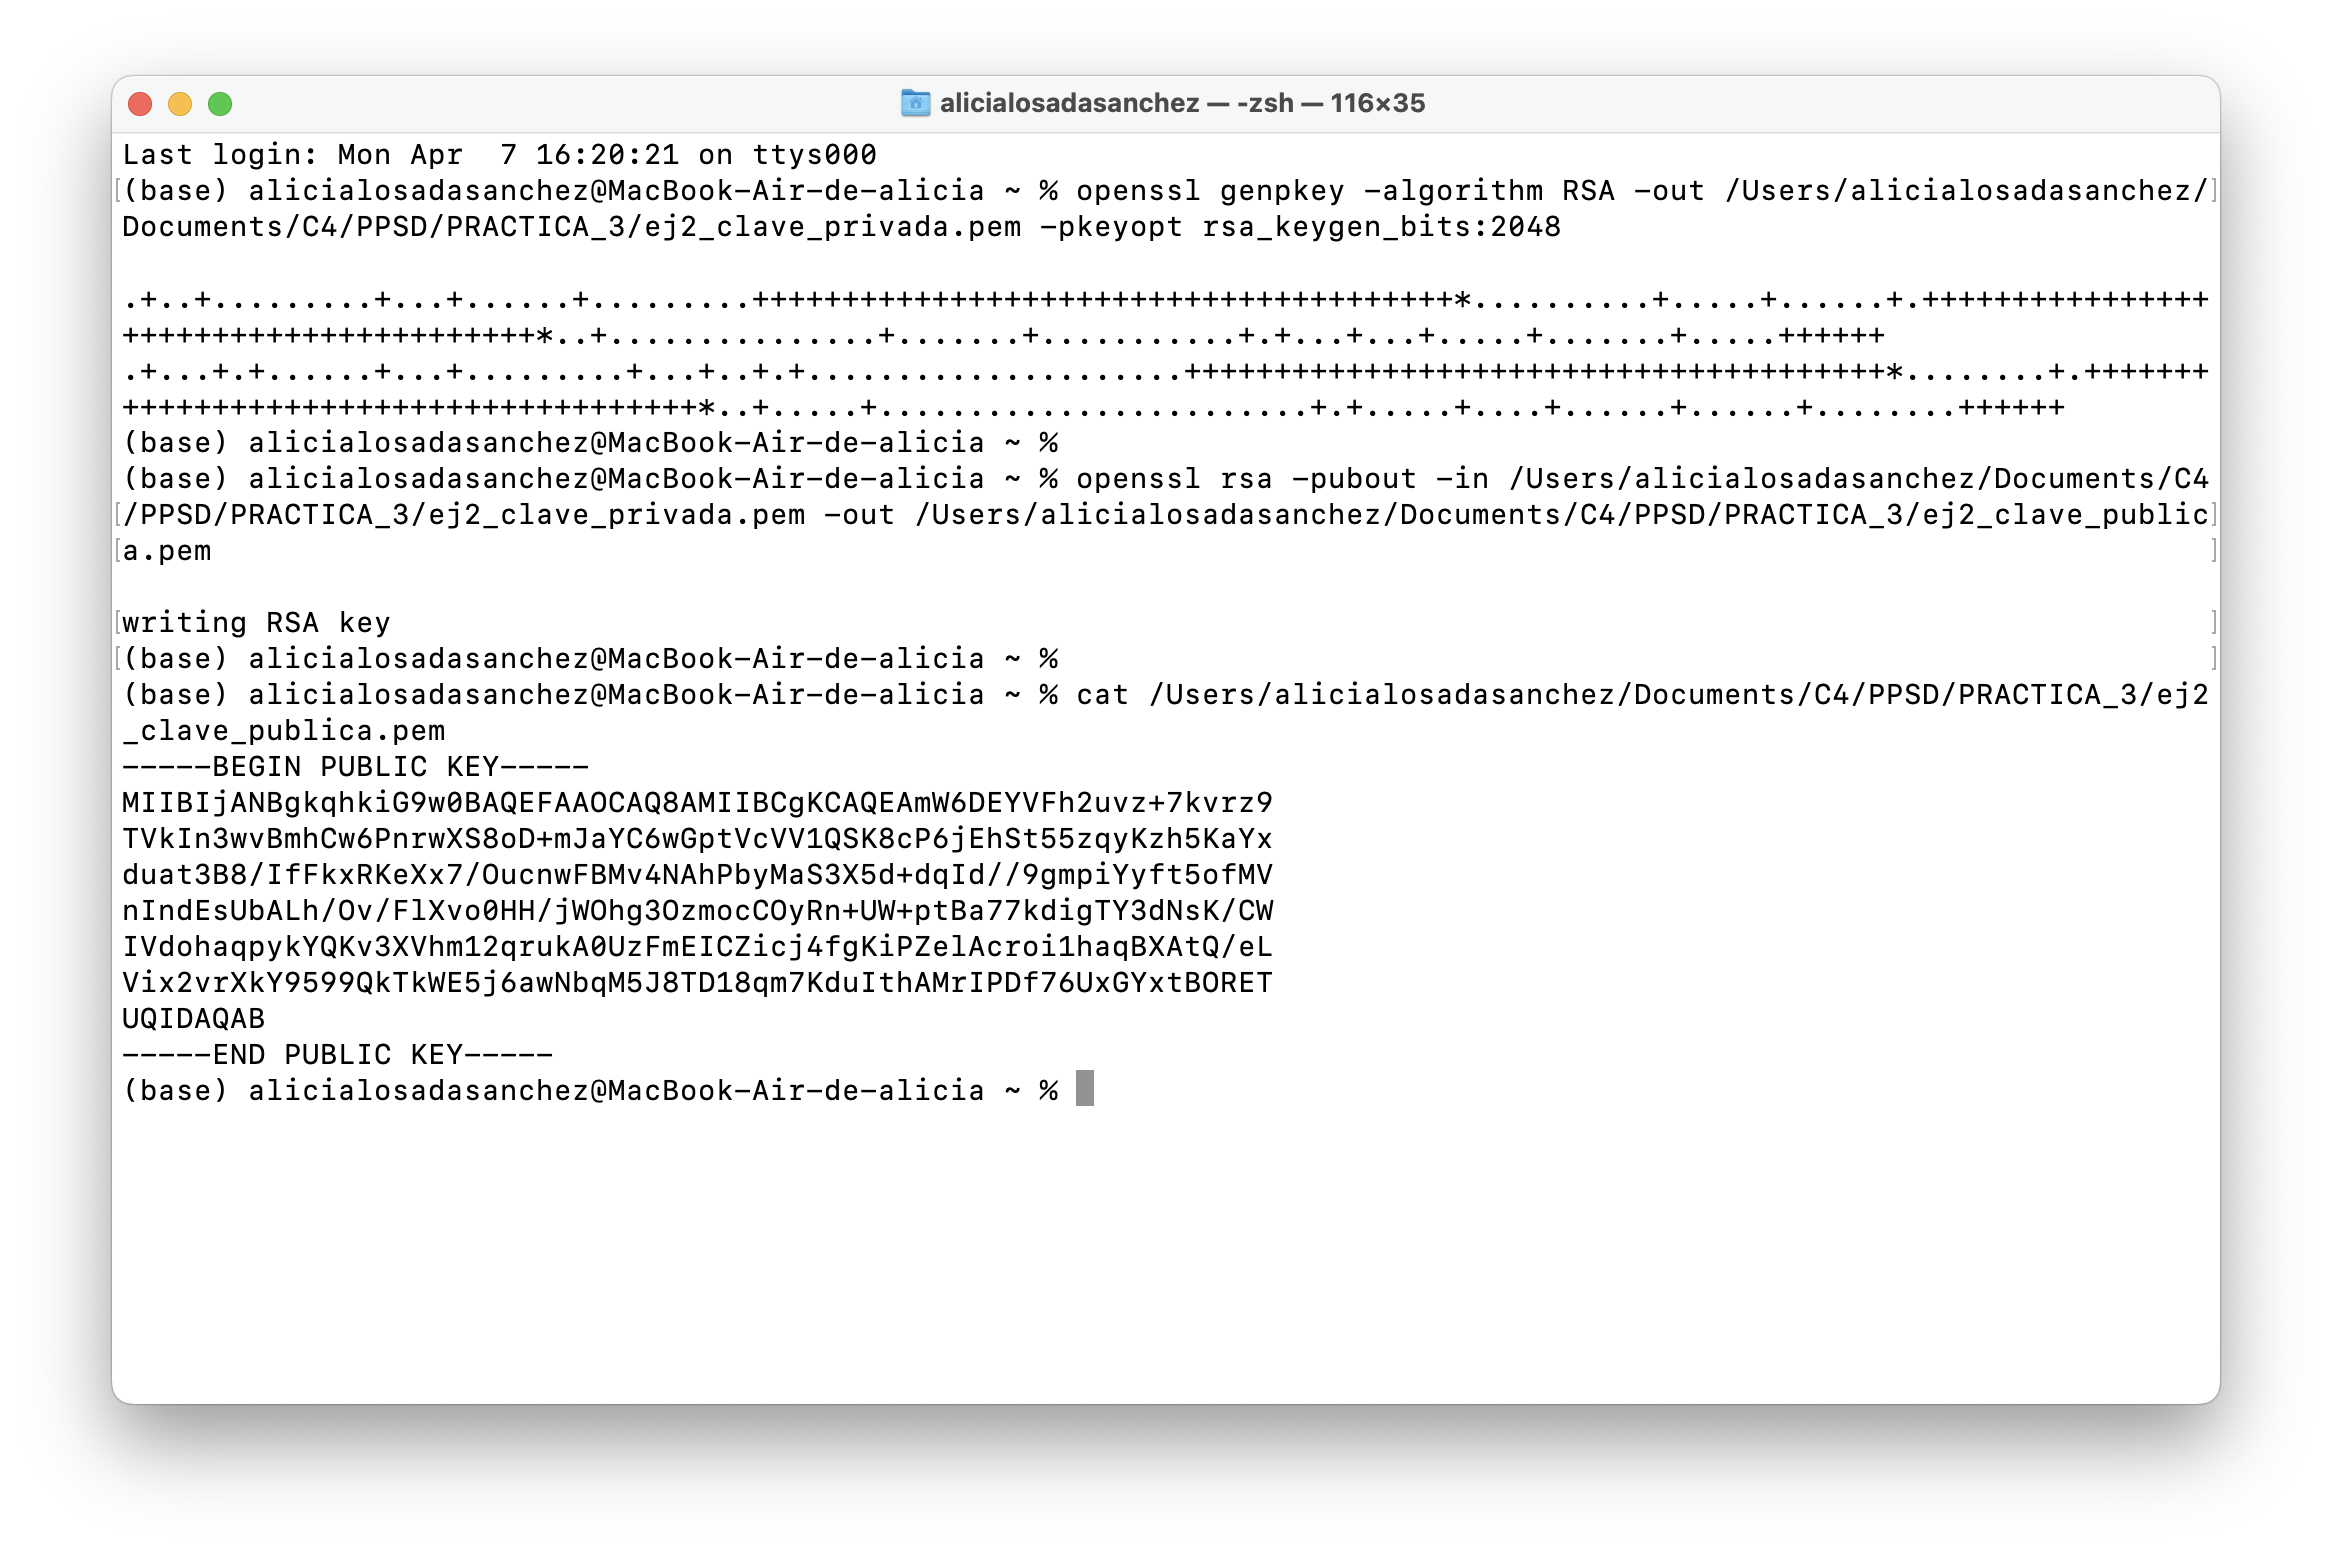
\includegraphics[width=15cm]{ej2_a.png}
    \caption{Generación clave RSA OpenSSL}
    \label{fig:generacion_rsa_openssl}
\end{figure}

Con el primer comando de la \ref{fig:generacion_rsa_openssl} generamos una clave privada de 2048 bits. Obtenemos la clave pública desde la clave privada con el segundo comando. En la \ref{fig:generacion_rsa_openssl} se puede ver el contenido de la clave pública. 


\subsubsection{¿Qué números conforman la clave pública?}

\begin{figure}[H]   
    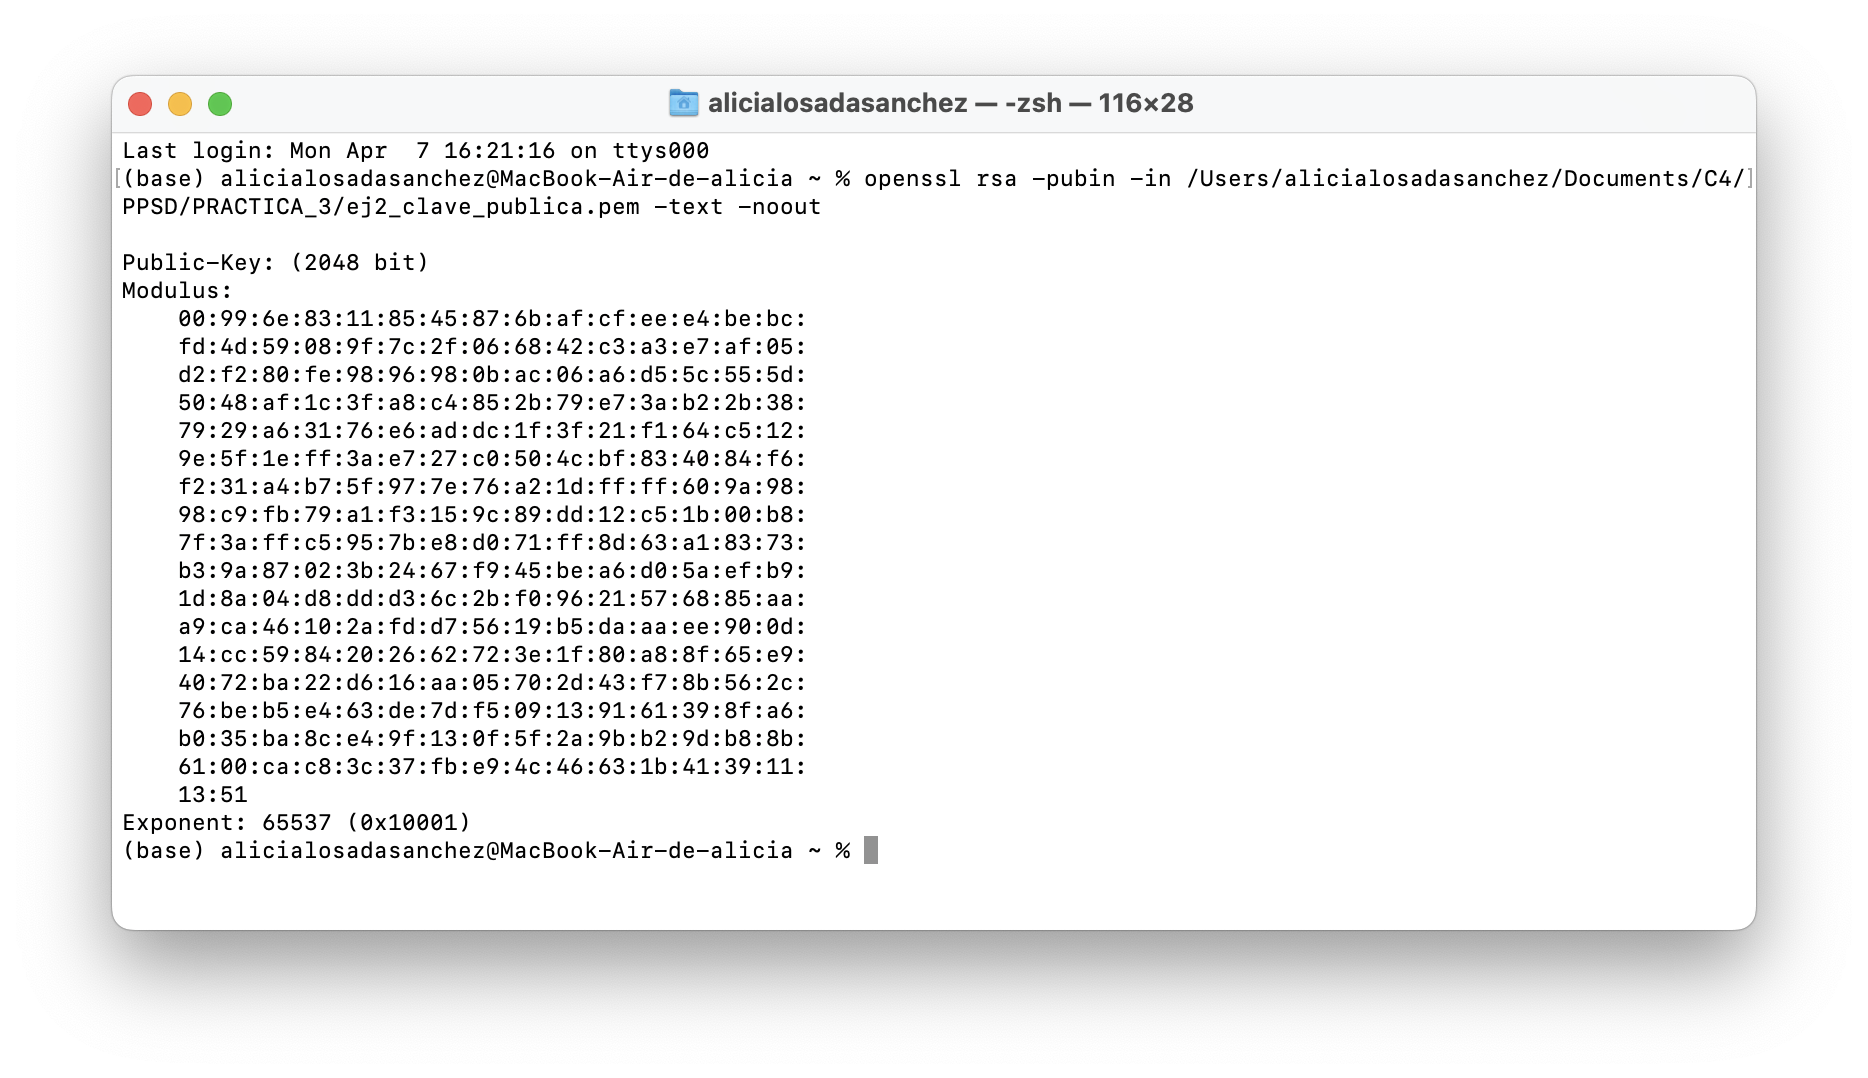
\includegraphics[width=15cm]{ej2_b.png}
    \caption{Partes clave pública}
    \label{fig:partes_clave_publica_rsa_openssl}
\end{figure}

Como se explica en el ejercicio 1, la clave pública está formada principalmente por dos números. El primero de ellos es el módulo ‘n’, que consiste en el producto de dos números primos (p y q vistos en las clases teóricas) y es común tanto a la clave pública como a la privada. El segundo es el exponente público ‘e’ que, como sucede en este caso, suele tomar el valor de 65537. En la \ref{fig:partes_clave_publica_rsa_openssl} se ve cuáles son esos valores para la clave previamente creada. 

\subsubsection{Cifrado secreto}

\begin{figure}[H]   
    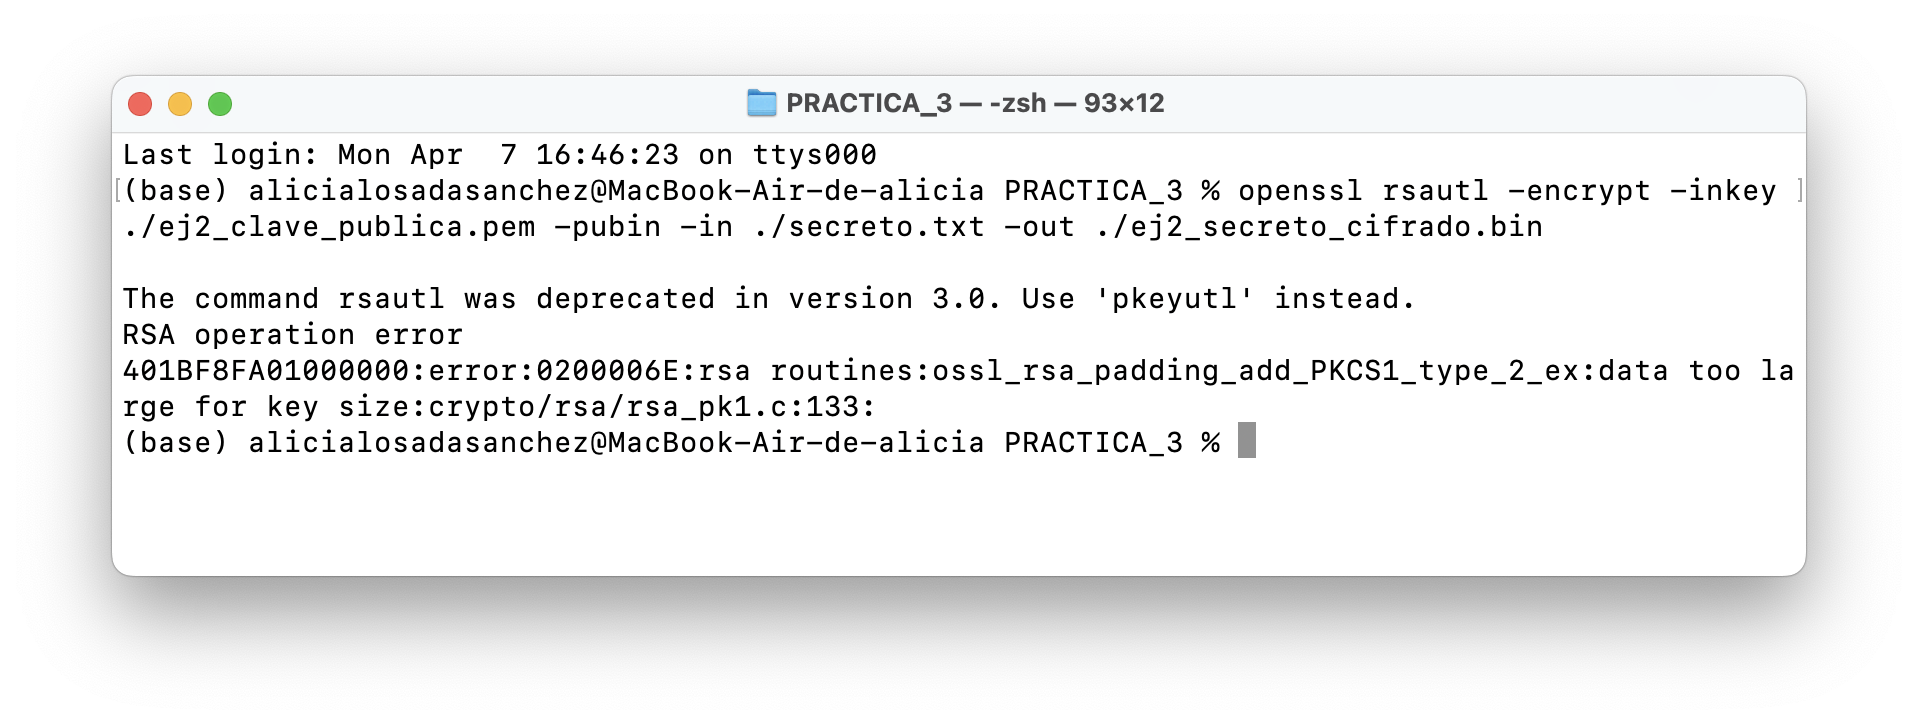
\includegraphics[width=15cm]{ej2_c.png}
    \caption{Cifrado secreto.txt}
    \label{fig:cifrado_secreto_openssl}
\end{figure}

El comando para cifrar el archivo secreto.txt con la clave pública generada se ve en la \ref{fig:cifrado_secreto_openssl}. Como se ve, obtuvimos una limitación al ejecutar el comando debido a que el tamaño del archivo.  

RSA es un algoritmo de cifrado asimétrico, diseñado para trabajar con bloques de datos pequeños. El archivo secreto.txt contiene más de 5000 caracteres, por lo que no es posible cifrarlo directamente con RSA. 

La solución que proponemos es llevar a cabo un cifrado mixto o híbrido, es decir, utilizar dos algoritmos de cifrado, uno simétrico y otro asimétrico. AES es un algoritmo de cifrado simétrico de bloques que permite el uso de claves de hasta 256 bits. 

Nuestra propuesta consiste en cifrar nuestro archivo secreto.txt con AES usando una clave secreta de 256 bits. Posteriormente, esta clave será la que se cifrará usando RSA, ya que sí cabe dentro del límite del algoritmo. 